This module deals with the main process behind STORM, it is the shuffling algorithm.
\begin{figure}[h]
	\centering
	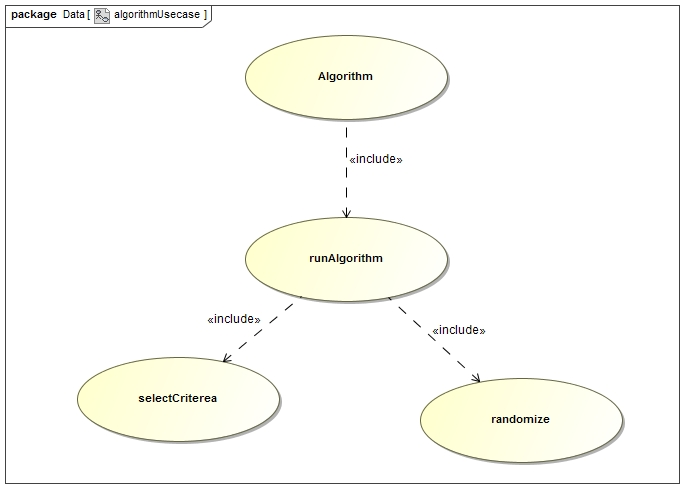
\includegraphics[width=15cm]{./graphics/algorithmUsecase.jpg}
	\caption{Algorithm module use case}
\end{figure}
\subsubsection{Use-cases}

The algorithm module adds the functionality required to shuffle subjects into teams.\par

\begin{enumerate}
\item Randomize\par
Priority: Critical.\par
Pre-condition: Project must have users.\par
Pre-condition: Team size or number of teams must be specified.\par
Post-condition: Random teams are built.\par
    \begin{figure}[h]
        \centering
        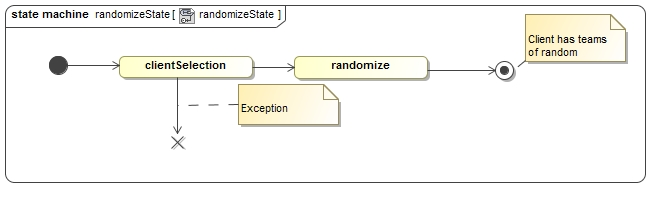
\includegraphics[width=15cm]{./graphics/randomizeState.jpg}
        \caption{Randomize state diagram}
    \end{figure}
\end{enumerate}
To be completed in future iterations
\pagebreak